\section{Additive Manufacturing}
As seen in figure \autoref{fig:am-methods-comparison}, coldspray manfuacturing is on the higher end of deposition rates, which is a key parameter for in-space manufacturing's ability to scale. [argue this better] The other methods that are higher than this are also great candidtates for in-space manfuacturing but have different drawbacks.
\begin{figure}[htbp]
    \centering

    \begin{minipage}{0.65\textwidth}
        \centering
        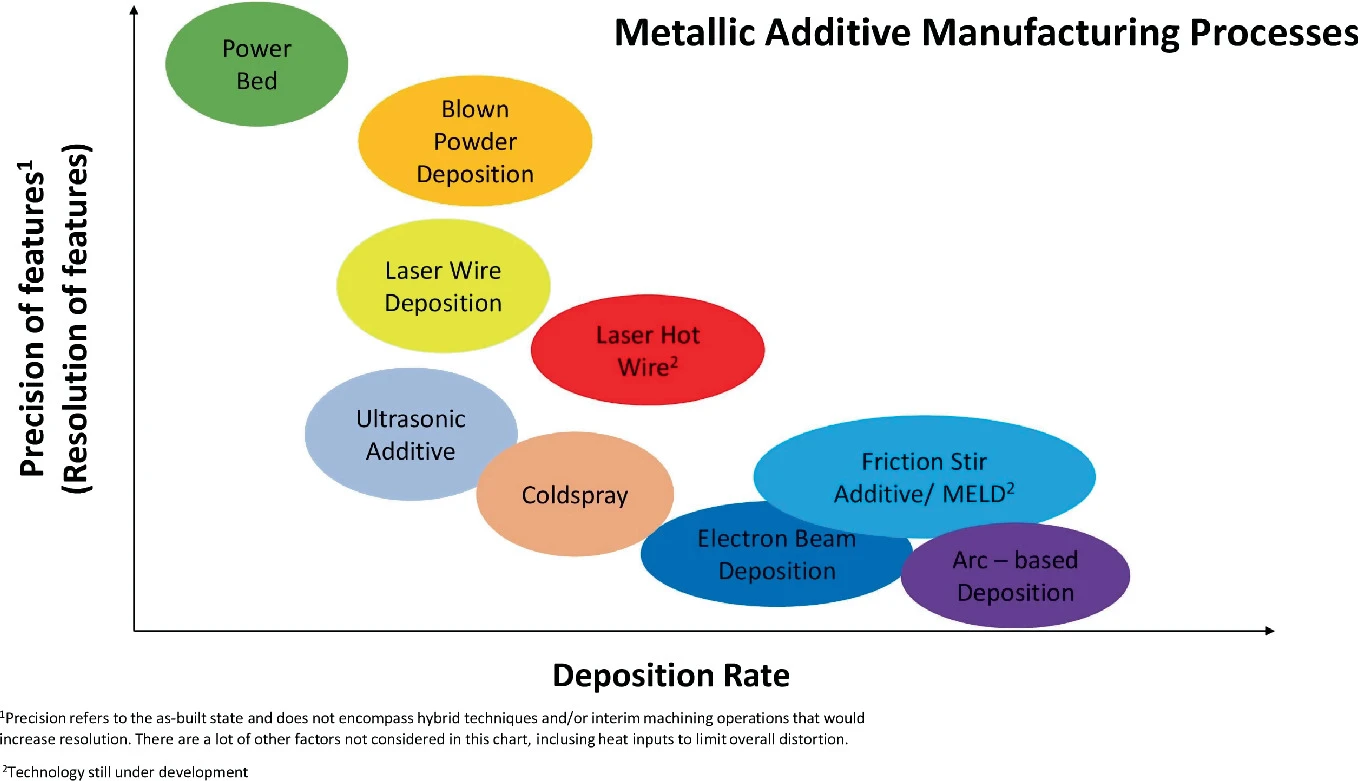
\includegraphics[width=\textwidth]{../report_assets/am-comparrison.png}
        \caption{Current feed system diagram\cite{Ramoni2022}.}\label{fig:am-methods-comparison}
    \end{minipage}

\end{figure}

Friction Stir Deposition (FSD) is a process that uses a rotating tool to create frictional heat and plastic deformation in the material, allowing it to be deposited onto a substrate. This process has a high deposition rate, but the need for a rotating tool, changover of this tool and the low technology readiness level (TRL) of 4\cite{nasa2025fsd} excludes it from benefiting much from research into its space applications at this stage.
Arc-based deposition methods, such as Wire Arc Additive Manufacturing (WAAM) have already been investigated for in-space applications and show great promise. However, these direct energy deposition (DED) methods are not suitable for all manufacturing applications due to melting the material, which can lead to residual stresses and distortion in the final part\cite{PATTISON2007627}. Laser Hot Wire and Electron Beam Melting also fall into this category but one could argue they are even less suitable due to geometry restrictions and additional system complexity respectively.


maybe talk about sls and other powder bed stuff


This leaves a gap in current research for a high deposition rate, non-thermal additive manufacturing process that is suitable for in-space applications. Cold Spray Additive Manufacturing (CSAM) is a promising candidate to fill this gap, as it has a high deposition rate, a wide range of materials available, and is non-thermal in nature. 

\section{Cold Spray}
CSAM works by accelerating metal powder particles to supersonic speeds using high velocity gas, causing them to deform and bond to a substrate. 

Any atomically-flat clean surfaces of metal will bond together when they come into contact in a vacuum\cite{holzbauer2024}. This is known as cold welding and works because the surface energy of the metals seperated is higher than that of them bonded together and so they move towards the lower energy state. The atoms undergo surface diffusion and rearrangement along their crystaline structures\cite{ctx46070057700001591} to form this metallic bond. 

While the particles themselves are often coated in an oxide layer, the high velocity of the impact causes the oxide layer to be removed, exposing the clean metal surface underneath. This is thought to be caused by adiabatic shear instability at the interface that breaks up the layer\cite{assadi2016cold}. This is a key feature of cold spray, as it allows for the bonding of materials that would otherwise be difficult to weld or bond together.


While it is debated in literature the exact nature of this deformation ...
As the particle impacts the substrate, it undergoes compaction into the substrate as well as metallurgically bonding over a significant portion of the contact area.
\subsection{Core Process}
When a particle is accelerated to a high velocity, it undergoes plastic deformation upon impact with the substrate. This deformation causes the particles to bond together, creating a solid layer of material. 

key parameters
\subsection{Advantages}
compare to other am techniques
\subsection{Space Applications}

gaps in research

\section{COSMOS}
aims, objectives, results and limitations